\documentclass[convert]{standalone}


\usepackage{tikz}
\usepackage{ifthen}

\tikzstyle{dots}=[%
	every node/.style={
		circle, inner sep = 0, fill=black, minimum size = 3pt, anchor=south
	}%
]

\begin{document}
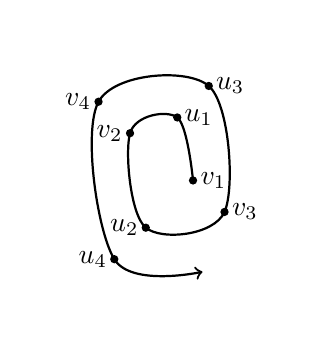
\begin{tikzpicture}[scale=0.2, dots]
	\draw[fill=white, draw=none] (-8.5,-11.5) rectangle ++(17,19.5);

	\node[label={right:{$u_1$}}] (u1) at (1,2)  {};
	\node[label={right:{$u_3$}}] (u3) at (3,4) {};

	\node[label={left:{$u_2$}}] (u2) at (-1,-5) {};
	\node[label={left:{$u_4$}}] (u4) at (-3,-7) {};
	
	\node[label={right:{$v_1$}}] (v1) at (2,-2) {};
	\node[label={right:{$v_3$}}] (v3) at (4,-4) {};
	
	\node[label={left:{$v_2$}}] (v2) at (-2,1) {};
	\node[label={left:{$v_4$}}] (v4) at (-4,3) {};

	\draw [thick, black, ->] plot [smooth, tension=0.6] coordinates {
		(v1) (u1) %
		(v2) (u2)%
		(v3) (u3)%
		(v4) (u4)%
		(2.6,-7.5)%
		% (3.8,-10)%
		% (5,-12.5)%
	};
\end{tikzpicture}
\end{document}








